\documentclass{beamer}

\usepackage{beamerthemesplit} %Activate for custom appearance
\usepackage{wrapfig}
\usepackage{amsmath}
\usepackage{amsfonts}
\usepackage{amssymb}
\usepackage{amsthm}
%\usepackage[outdir=./]{epstopdf}
\usepackage{mathbbol}
%\usepackage{tikz}
\usepackage{color}
\usepackage[ruled]{algorithm}
\usepackage{algorithmic}
\usepackage{multirow}
\usepackage{graphicx}
\usepackage{xkeyval}
\usepackage{todonotes}
\presetkeys{todonotes}{inline}{}
\usepackage{arydshln}
\usepackage{caption} 
\usepackage{subcaption}
\usepackage{verbatim}
\usepackage[update,prepend]{epstopdf}
\definecolor{DeepSkyBlue}{rgb}{0.6,0.6,1}
\setbeamercolor{eecks} {bg=DeepSkyBlue, fg=black!10}
\setbeamercolor{eeks2}{bg=black!8, fg=black}

\mode<presentation>{%
  \usetheme{Boadilla}
}

\usefonttheme[onlymath]{serif}
\newenvironment{ovalboxpage}[1]{\begin{center}\begin{minipage}{#1}\begin{block}{}}{\end{block}\end{minipage}\end{center}}
\newenvironment{ovalboxpagetitle}[2]{\begin{center}\begin{minipage}{#1}\begin{block}{#2}}{\end{block}\end{minipage}\end{center}}
\newenvironment{obpt}[1]{\begin{center}\begin{minipage}{0.95\textwidth}\begin{block}{#1}}{\end{block}\end{minipage}\end{center}}
\newenvironment{obptsmall}[1]{\begin{center}\begin{minipage}{0.6\textwidth}\begin{block}{#1}}{\end{block}\end{minipage}\end{center}}

\newcommand{\R}{\mathbb{R}}

\title[Fast Somewhat Accurate Algorithms]{Fast and Somewhat Accurate Algorithms (Team 4)}
\author[Team 4]{Mario Barela, Su Chen,
Emily Gunawan,
Morgan Schreffler, Minho Song,
Doyeob Yeo, with mentor:
Chai Wah Wu (IBM)}
\date[Final Presentation]{Friday, August 14, 2015}
\institute[IMA]{IMA: Modeling in Industry Final Presentation}

\begin{document}
\begin{frame}
\titlepage % Print the title page as the first slide
\end{frame}


\begin{frame}
\frametitle{Outline}
  \begin{figure}[htb]
  \begin{center}
  \mbox{\includegraphics[height=1in]{BaboonRGB.jpg}}
\mbox{\includegraphics[height=1in]{Baboon_after_sobel_magnitude.jpg}}
\mbox{\includegraphics[height=1in]{Baboon_after_sobel_magnitude_inverse.jpg}}
  % Mandrill 
 
  \end{center}
  \end{figure}
% Table of contents slide, comment this block out to remove it

\tableofcontents % Throughout your presentation, if you choose to use \section{} and \subsection{} commands, these will automatically be printed on this slide as an overview of your presentation
\end{frame}

\section{Motivation/Problem}

\begin{frame}
\frametitle{Problem}
We study the tradeoff between accuracy and system complexity as measured by processing speed and hardware complexity.

\end{frame}

\begin{comment}
\begin{frame}
\frametitle{Where is image processing used?}
\begin{figure}[htb]
  \begin{center}  \mbox{\includegraphics[height=1in]{Quality_Control.jpg}}
   \mbox{\includegraphics[height=1in]{Quality_Control_after_sobel_magnitude.jpg}}
 \mbox{\includegraphics[height=1in]{Quality_Control_after_sobel_magnitude_inverse.jpg}}
  \caption{Pastry industry quality control}
  \end{center}
  \end{figure}
  
\begin{itemize}
%\item Quality Control 
\item
Computer vision (license plate reader, tracking human motion)
\item
Optical imaging (cameras, microscopes)
\item
Medical imaging (MRI, ultrasound) %, %astronomical imaging (telescopes)
\item
Geophysical imaging, printing
\end{itemize}
\end{frame}

\section{Filtering an Image}

\begin{frame}
\frametitle{An edge-detection filter example}

\todo{Emily writes: this slide is not necessary. To save time, this slide can be removed/replaced.}
\begin{figure}[htb]
  \begin{center}
  \mbox{\includegraphics[height=1in]{german.png}}
   \mbox{\includegraphics[height=1in]{german_after_sobel_magnitude.png}}
   
 \mbox{\includegraphics[height=1in]{german_after_sobel_magnitude_inverse.png}}  
%  \caption{German houses from Kodak}
  \end{center}
\end{figure}

\end{frame}


\begin{frame}
\frametitle{Kernel Convolution $\text{IMAGE}*K$}
\todo{Emily writes: I think this slide (and the next one) is not the best. I don't care if this slide (and the next slide) is removed/replaced.}

\begin{itemize}
\item A \emph{convolution matrix} % or kernel, or mask
is a small matrix used for filtering an image.
\item $\text{IMAGE}=
\begin{bmatrix}
\textcolor{blue}{a} & \textcolor{blue}{b} & \textcolor{blue}{c} & d \\
\textcolor{blue}{e} & \textcolor{red}{g} & \textcolor{blue}{h} & i\\
\textcolor{blue}{j} & \textcolor{blue}{m} & \textcolor{blue}{n} & p
\end{bmatrix}$
and
$
K = \begin{bmatrix}
{0} & {-1} & {0}\\
{-1} & {4} & -1\\
{0} & {-1} & {0}
\end{bmatrix}$

\item %To compute the new pixel value at the location of \textcolor{red}{$g$},
%we put the flipped kernel $F$ on top of
To compute the new value at pixel % at the location of
\textcolor{red}{$g$},
place $K$ on top of 
$\text{IMAGE}$, centered at $\textcolor{red}{g}$.
Perform point-wise multiplications and sum up the results:\\

$\begin{bmatrix}
0(a) & -1(b) & 0(c) \\
-1(e) & 4\textcolor{red}{(g)} & -1(h) \\
0(j) & -1(m) & 0(n) 
\end{bmatrix}$

\bigskip

\item The pixel \textcolor{red}{$g$} is replaced by:
$-b-e+4\textcolor{red}{g}-h-m.$

\end{itemize}
\end{frame}


\begin{frame}
\frametitle{Kernel Convolution $\text{IMAGE}*K$}
%$IMAGE
$
\tiny
\begin{bmatrix}
\textcolor{blue}{a} & \textcolor{blue}{b} & \textcolor{blue}{c} & d \\
\textcolor{blue}{e} & \textcolor{red}{g} & \textcolor{blue}{h} & i\\
\textcolor{blue}{j} & \textcolor{blue}{m} & \textcolor{blue}{n} & p
\end{bmatrix}
*\tiny{\begin{bmatrix}
0 & -1 & 0\\
-1 & 4 & -1\\
0 & -1 & 0
\end{bmatrix}}=$
\tiny
 \[
\arraycolsep=0.6pt\def\arraystretch{2.9}
\left[ 
\begin{array}{c@{}c@{}c@{}c}
\begin{array}{ccccc}
0(0) &+& 0(-1) &+& 0(0)+\\ 
0(-1) &+& a(4) &+& b(-1)+\\
0(0) &+& e(-1) &+& g(0)\\
\end{array}
  & 
\left| \begin{array}{ccccc}
0(0) &+& 0(-1) &+& 0(0)+\\ 
a(-1) &+& b(4) &+& c(-1)+\\
e(0) &+& g(-1) &+& h(0)\\
\end{array}\right| 
  & 
\begin{array}{ccccc}
0(0) &+& 0(-1) &+& 0(0)+\\ 
g(-1) &+& h(4) &+& i(-1)+\\
m(0) &+& n(-1) &+& p(0)\\
\end{array} 
  & 
  \left|
\begin{array}{ccccc}
0(0) &+& 0(-1) &+& 0(0)+\\ 
h(-1) &+& i(4) &+& 0(-1)+\\
n(0) &+& p(-1) &+& 0(0)\\
\end{array} 
\right|
\\ \hdashline % end of first row
\begin{array}{ccccc}
0(0) &+& a(-1) &+& b(0) +\\ 
0(-1) &+& e(4) &+& g(-1) +\\
0(0) &+& j(-1) &+& m(0) \\
\end{array} 
&
\left|  
\textcolor{red}{
\begin{array}{ccccc}
a(0) &+& b(-1) &+& c(0) +\\ 
e(-1) &+& g(4) &+& h(-1) +\\
j(0) &+& m(-1) &+& n(0) \\
\end{array}}\right| 
& 
\textcolor{black}{
\begin{array}{ccccc}
b(0) &+& c(-1) &+& d(0) +\\ 
g(-1) &+& h(4) &+& i(-1) +\\
m(0) &+& n(-1) &+& p(0) \\
\end{array} }
& 
\left|
\begin{array}{ccccc}
c(0) &+& d(-1) &+& 0(0) +\\ 
h(-1) &+& i(4) &+& 0(-1) +\\
n(0) &+& p(-1) &+& 0(0)\\
\end{array} 
\right|
\\ \hdashline % end of second row
\begin{array}{ccccc}
0(0) &+& e(-1) &+& g(0) +\\ 
0(-1) &+& j(4) &+& m(-1) +\\
0(0) &+& 0(-1) &+& 0(0)\\
\end{array} 
& 
\left| \begin{array}{ccccc}
e(0) &+& g(-1) &+& h(0) +\\ 
j(-1) &+& m(4) &+& n(-1) +\\
0(0) &+& 0(-1) &+& 0(0) \\
\end{array} \right| 
&
\begin{array}{ccccc}
g(0) &+& h(-1) &+& i(0) +\\ 
m(-1) &+& n(4) &+& p(-1) +\\
0(0) &+& 0(-1) &+& 0(0) \\
\end{array} 
&
\left|
\begin{array}{ccccc}
h(0) &+& i(-1) &+& 0(0) +\\ 
n(-1) &+& p(4) &+& 0(-1) +\\
0(0) &+& 0(-1) &+& 0(0)\\
\end{array} 
\right|
\end{array} 
\right]
\]    
  \end{frame}
%%%
\end{comment}



\section{Strategies for faster algorithms}

\begin{frame}
\frametitle{Strategies to Simplify Computations in Image Filtering}
\begin{figure}[htb]
  \begin{center}
  \includegraphics[height=1.5in]{FOCUS.JPG}
  
  \end{center}
  \end{figure}
\begin{enumerate}
\item Use lookup tables (LUTs) to reduce computation time
\pause\item Use bit truncation to reduce the size of LUTs
\pause\item Decompose kernel exactly or approximately to simplify LUTs
\end{enumerate}
\end{frame}

\begin{frame}
\frametitle{Reduce Processing Time Using Look-up Tables (LUTs)}
\begin{beamerboxesrounded}[lower=eeks2,upper=eecks,
shadow=true]{IDEA}
%Idea: %Store the pre-calculated 
Prior to applying filter,
pre-compute convolutions for all possible square matrices and 
store them in a multi-dimensional table.
%and retrieve them directly when applying to an image.
\end{beamerboxesrounded}

$$
K * \begin{bmatrix}
x_1 & x_2 & x_3\\
x_4 & x_5 & x_6\\
x_7 & x_8 & x_9
\end{bmatrix}
 \rightarrow LUT(x_1,x_2,\dots,x_9)
$$

\begin{itemize}
\item Save time by retrieving the values in $LUT(x_1,\dots,x_9)$ (in place of direct algebraic computations).
\item Challenge: a full-size LUT for a $3 \times 3$ kernel requires $2^{72}$ bytes (assuming each pixel is 8 bits).
\end{itemize}
\end{frame}

\begin{frame}\frametitle{Truncating to Reduce LUT Size}
\begin{beamerboxesrounded}[lower=eeks2,upper=eecks,
shadow=true]{IDEA}
If we reduce the number of possible inputs, we can reduce the number of elements in the LUT!
\end{beamerboxesrounded}

\pause\begin{solution}Replace the inputs

\[
\left.
\begin{matrix}
 40 = &00101\underline{000}\\
 &00101\underline{001}\\
 &00101\underline{010}\\
 &00101\underline{011}\\
 &00101\underline{100}\\
 &00101\underline{101}\\
 &00101\underline{110}\\
 47 = &00101\underline{111} 
 \end{matrix}
\right\}
\text{ with }\longrightarrow
00101\underline{100}
\]

to do the kernel convolution, and pre-store the results in the LUT with index $00101$.
\end{solution}

\end{frame}

\begin{frame}\frametitle{Truncation Matrices and Image Norms}
If our convolution kernel $K$ is $n\times n$, we can choose a \emph{truncation matrix} $T = [t_{ij}]_{n\times n}$ with integer elements from 0 to 8 to indicate how many bits to truncate from each pixel when convolving with $K$. An example might be $T = \left[\begin{smallmatrix}5 & 5 & 5\\ 5 & 2 & 5\\ 5 & 5 & 5\end{smallmatrix}\right]$

%\pause\begin{example}
%If $T = \left[\begin{smallmatrix}5 & 5 & 5\\ 5 & 2 & 5\\ 5 & 5 & 5\end{smallmatrix}\right]$, this indicates that before performing the computation for pixel $ij$, $ij$'s neighboring pixels' values should be truncated by 5 bits and pixel $ij$'s value should be truncated by 2 bits.
%\end{example}

\pause\begin{definition}[Image Norms]
\begin{itemize}
\item[]
$l_{\infty}$-error(A,B)$=\textrm{max}_{i,j} | a_{ij} - b_{ij}|$
\item[]
$l_2$-error(A,B)$=\sqrt{ \frac{ \sum_{i,j} \left( a_{ij} - b_{ij} \right)^2} {h \times w}}$
\item []
PSNR(A,B)$=20 \cdot \textrm{log}_{10} ( \frac{\textrm{MAX}_B}{\sqrt{\textrm{MSE}}} )$
\item[] $d_\text{IMED}^2(A,B) = \frac{1}{2\pi\cdot h\cdot w}\sum_{i,k = 1}^h\sum_{j,\ell = 1}^w \exp\left(\frac{-(k^2+\ell^2)}{2}\right)\big(a_{ij}-b_{ij}\big)\big(a_{i+k,j+\ell} - b_{i+k,j+\ell}\big)$
\end{itemize}
\end{definition}
\end{frame}

\begin{frame}\frametitle{High Pass Filters: Direct Computation vs. Truncation}
\begin{center}
\only<1>{For the next few slides, we will consider these birds.
\includegraphics[scale=.64]{gulls/gulls.png}}
%\only<2>{Here they are in grayscale.
%\includegraphics[scale=.31]{gulls/fig01_gulls_gray.eps}}
\end{center}
\end{frame}

\begin{frame}\frametitle{Example 1 of a $3\times3$ High Pass Filter}
\begin{center}
\only<1>{This is them after the HP kernel $K_1 = \frac14\left[\begin{smallmatrix}0 & \text{-}1 & 0\\\text{-}1 & 4 & \text{-}1\\0 & \text{-}1 & 0\end{smallmatrix}\right]$ was applied.
\includegraphics[scale=.31]{gulls/fig02_HP_3x3_dc_1-eps-converted-to.pdf}}
\only<2>{C'mon baby, make it HOT!
\includegraphics[scale=.31]{gulls/fig02_HP_3x3_dc_1_HOT-eps-converted-to.pdf}}
\only<3>{Here they are with $K_1$ applied with truncation $T_1 = \left[\begin{smallmatrix}8 & 3 & 8\\3 & 1 & 3\\8 & 3 & 8\end{smallmatrix}\right]$.
\includegraphics[scale=.31]{gulls/fig03_HP_3x3_trunc_1_HOT-eps-converted-to.pdf}}
\only<4>{Here is the difference image, color-coded for convenience.
\includegraphics[scale=.47,clip,trim = 0cm 4cm 0cm 4.5cm]{gulls/fig04_HP_3x3_trunc_vs_dc_1-eps-converted-to.pdf}}
\end{center}
\only<4>{\vspace{-1cm}\hspace{1.8cm}\large{0} \hspace{.58cm}\large{1} \hspace{.58cm}\large{2} \hspace{.58cm}\large{3} \hspace{.56cm}\large{4} \hspace{.58cm}\large{5} \hspace{.58cm}\large{6} \hspace{.56cm}\large{7} \hspace{.58cm}\large{8} \hspace{.56cm}\large{9}}
\end{frame}

\begin{frame}\frametitle{Example 2 of a $3\times3$ High Pass Filter}
\begin{center}
\only<1>{This is the gulls after the HP kernel $K_2 = \frac18\left[\begin{smallmatrix}\text{-}1 & \text{-}1 & \text{-}1\\\text{-}1 & 8 & \text{-}1\\\text{-}1 & \text{-}1 & \text{-}1\end{smallmatrix}\right]$ was applied.
\includegraphics[scale=.31]{gulls/fig08_HP_3x3_dc_2_HOT-eps-converted-to.pdf}}
\only<2>{Here they are with $K_1$ applied with truncation $T_2 = \left[\begin{smallmatrix}4 & 4 & 4\\4 & 1 & 4\\4 & 4 & 4\end{smallmatrix}\right]$.
\includegraphics[scale=.31]{gulls/fig09_HP_3x3_trunc_2_HOT-eps-converted-to.pdf}}
\only<3>{Here is the difference image, color-coded for convenience.
\includegraphics[scale=.47,clip,trim = 0cm 4cm 0cm 4.5cm]{gulls/fig10_HP_3x3_trunc_vs_dc_2-eps-converted-to.pdf}}
\end{center}
\only<3>{\vspace{-1cm}\hspace{1.8cm}\large{0} \hspace{.668cm}\large{1} \hspace{.666cm}\large{2} \hspace{.668cm}\large{3} \hspace{.666cm}\large{4} \hspace{.668cm}\large{5} \hspace{.668cm}\large{6} \hspace{.666cm}\large{7} \hspace{.668cm}\large{8}}
\end{frame}

\begin{frame}\frametitle{Example of a $5\times5$ High Pass Filter}
\begin{center}
\only<1>{This is the gulls after the HP kernel $K_3 = \frac{1}{24}\left[\begin{smallmatrix}\text{-}1 & \text{-}1 & \text{-}1 & \text{-}1 & \text{-}1\\\text{-}1 & \text{-}1 & \text{-}1 & \text{-}1 & \text{-}1\\\text{-}1 & \text{-}1 & 24 & \text{-}1 & \text{-}1\\\text{-}1 & \text{-}1 & \text{-}1 & \text{-}1 & \text{-}1\\\text{-}1 & \text{-}1 & \text{-}1 & \text{-}1 & \text{-}1\\\end{smallmatrix}\right]$.
\includegraphics[scale=.3]{gulls/fig05_HP_5x5_dc_HOT-eps-converted-to.pdf}}
\only<2>{Here they are with $K_3$ applied with truncation $T_3 = \left[\begin{smallmatrix}5 & 5 & 5 & 5 & 5\\5 & 5 & 5 & 5 & 5\\5 & 5 & 1 & 5 & 5\\5 & 5 & 5 & 5 & 5\\5 & 5 & 5 & 5 & 5\\\end{smallmatrix}\right]$.
\includegraphics[scale=.3]{gulls/fig06_HP_5x5_trunc_HOT-eps-converted-to.pdf}}
\only<3>{Here is the difference image, color-coded for convenience.
\includegraphics[scale=.31,clip,trim = 0cm 1cm 0cm 1cm]{gulls/fig07_HP_5x5_trunc_vs_dc-eps-converted-to.pdf}}
\end{center}
\onslide<3>{\vspace*{-.75cm}\hspace{1.8cm}\large{0} \hspace{.625cm}\large{2} \hspace{.685cm}\large{4} \hspace{.685cm}\large{6} \hspace{.685cm}\large{8} \hspace{.685cm}\large{10} \hspace{.5cm}\large{12} \hspace{.5cm}\large{14} \hspace{.5cm}\large{16}}
\end{frame}

\begin{frame}\frametitle{And the Data to Back it Up!}
Here are three very different pictures.
\begin{figure}[h]
\begin{subfigure}[t]{0.3\textwidth}
\includegraphics[scale=.1]{lighthouse.jpg}
\caption{A lighthouse}
\end{subfigure}
\begin{subfigure}[t]{0.3\textwidth}
\includegraphics[scale=.1]{sunset.jpg}
\caption{A sunset}
\end{subfigure}
\begin{subfigure}[t]{0.3\textwidth}
\includegraphics[scale=.1]{waterfall.jpg}
\caption{A waterfall}
\end{subfigure}
\end{figure}
\pause When converted to grayscale and compared, we have the following chart:
\begin{table}[ht]
\begin{center}
\begin{tabular}{c|c|c|c|c|}\cline{2-5}
& $\ell^2$ & $\ell^\infty$ & PSNR & $d_\text{IMED}$ \\\hline \multicolumn{1}{ |c| }{(a) vs. (b)}
& 64.8743  & 251 & 9.3835 & 64.043 \\\hline
\multicolumn{1}{ |c| }{(a) vs. (c)}  & 59.2807 & 247 & 7.7803  & 58.6937\\\hline \multicolumn{1}{ |c| }{(b) vs. (c)} & 36.9946  & 229 & 10.3046 & 36.4582\\
\hline
\end{tabular}
\caption{Comparison of image distances}
%\label{table:comparison_of_errors}
\end{center}
\end{table}
\end{frame}

\begin{frame}\frametitle{And the Data to Back it Up!}
\begin{table}[ht]
\begin{center}
\begin{tabular}{c|c|c|c|c|}\cline{2-5}
& $\ell^2$ & $\ell^\infty$ & PSNR & $d_\text{IMED}$ \\\hline \multicolumn{1}{ |c| }{(a) vs. (b)}
& 64.8743  & 251 & 9.3835 & 64.043 \\\hline
\multicolumn{1}{ |c| }{(a) vs. (c)}  & 59.2807 & 247 & 7.7803  & 58.6937\\\hline \multicolumn{1}{ |c| }{(b) vs. (c)} & 36.9946  & 229 & 10.3046 & 36.4582\\
\hline
\end{tabular}
%\caption{Comparison of image distances}
%\label{table:comparison_of_errors}
\end{center}
\end{table}
Keep these numbers in mind as we compare our filtered images.

\pause\begin{table}[ht]
\begin{center}
\begin{tabular}{c|c|c|c|c|}\cline{2-5}
& $\ell^2$ & $\ell^\infty$ & \only<2>{PSNR} \only<3>{\textcolor{red}{PSNR}} & $d_\text{IMED}$ \\\hline \multicolumn{1}{ |c| }{$K_1$ DC vs. $K_1$ Trunc.}
& 3.4992  & 9 & \only<2>{37.2515} \only<3>{\textcolor{red}{37.2515}} & 3.1401 \\\hline
\multicolumn{1}{ |c| }{$K_2$ DC vs. $K_2$ Trunc.}  & 3.6366 & 8 & \only<2>{36.917} \only<3>{\textcolor{red}{36.917}} & 3.3553\\\hline \multicolumn{1}{ |c| }{$K_3$ DC vs. $K_3$ Trunc.} & 8.5556  & 16 & \only<2>{29.4858} \only<3>{\textcolor{red}{29.4858}} & 8.2883\\
\hline
\end{tabular}
\caption{Comparison of filters and their truncated forms}
%\label{table:comparison_of_errors}
\end{center}
\end{table}
\pause The PSNR values are particularly indicative of acceptable error, since lossy compression typically has a PSNR of about 30-50.
\end{frame}

\begin{frame}
\frametitle{Decomposing rank 1 matrix}

\begin{beamerboxesrounded}[lower=eeks2,upper=eecks,
shadow=true]{IDEA}
%Idea: 
If the kernel $(n\times n)$ matrix $K$ has rank 1, then % we can write it as
$$
K=c\cdot b^T=c*b^T
$$
where $c,b\in \mathbb{R}^{n\times 1}$. For example,
\end{beamerboxesrounded}
$$
K=
\begin{bmatrix}
1 & 2 & 1\\
2 & 4 & 2\\
1 & 2 & 1
\end{bmatrix}
=
\begin{bmatrix}
1 \\
2 \\
1 
\end{bmatrix}
*
\begin{bmatrix}
1 & 2 & 1
\end{bmatrix}
$$
Applying a filter K to an Image then becomes
$$\text{IMAGE}*K=\text{IMAGE}*(c*b^T)=(\text{IMAGE}*c)*b^T
$$
so that we need two LUTs (with b and c) for one convolution.
\end{frame}



\begin{frame}
\frametitle{Decomposing rank 1 matrix}
An example: low pass filter with kernel
$$
K=\frac{1}{16}
\begin{bmatrix}
1 & 2 & 1\\
2 & 4 & 2\\
1 & 2 & 1
\end{bmatrix}
=\frac{1}{4}
\begin{bmatrix}
1 \\
2 \\
1 
\end{bmatrix}
*\frac{1}{4}
\begin{bmatrix}
1 & 2 & 1
\end{bmatrix}
\triangleq c* c^T
$$
\\
Truncation matrix: 
$$
T_1=
\begin{bmatrix}
 2 \\
 1\\
 2
\end{bmatrix}
, \ \ \ \ \ \ 
T_2=
\begin{bmatrix}
 4 \\
 2\\
 4
\end{bmatrix}
$$
By symmetry, only one look up table is needed.
\begin{enumerate}
\item Step 1: Generate look up table for $c=[1\ \  2\ \  1]^T$.
\item Step 2: Convolve the image with $c$. 
\item Step 3: Convolve transpose of the image with $c$. 
\end{enumerate}
\end{frame}

\begin{frame}
\begin{figure}[h] \centering 
\begin{subfigure}[b]{0.4\textwidth} \includegraphics[width=\textwidth]{motor_original.png} \caption{Original image} %\label{fig:LPF} 
\end{subfigure}
\begin{subfigure}[b]{0.4\textwidth} \includegraphics[width=\textwidth]{motor_direct.png} \caption{Low pass, direct}\end{subfigure}

\begin{subfigure}[b]{0.4\textwidth} \includegraphics[width=\textwidth]{motor_lut_121.png} \caption{Low pass, LUT with $T_1$} %\label{fig:LPF} 
\end{subfigure}
\begin{subfigure}[b]{0.4\textwidth} \includegraphics[width=\textwidth]{motor_lut_242.png} \caption{Low pass, LUT with $T_2$} \end{subfigure}
\caption{Comparison of filtered images.}
%\label{fig:comp} 
\end{figure}
\end{frame}


\begin{frame}
\begin{center}
\begin{table}
	 
    \begin{tabular}{ | c | c| c |}
    \hline
    Scheme & LUT Size & PSNR (dB) \\ \hline
    LUT with $T_1$ & 512KB & 41.8459 \\ \hline
    LUT with $T_2$ & 16KB & 30.4442 \\ \hline   
    \end{tabular}
    \bigskip
    
    \caption{Error and size of LUT for LUTs with different truncation schemes.}
\end{table} \label{tbl:low_pass}
\end{center}

\begin{center}
\begin{table}
	
    \begin{tabular}{ | c | c | c | }
    \hline
    LUT Size & Best Truncation & PSNR (dB) \\ \hline
    16KB& $(0,b,0)$ with $b=(4,2,4)^T$ & 30.4442 \\ \hline
    32KB& $(0,b,0)$ with $b=(3,3,3)^T$ & 33.3275 \\ \hline 
    64KB& $(0,b,0)$ with $b=(3,2,3)^T$ & 35.5597 \\ \hline 
    256KB& $(0,b,0)$ with $b=(2,2,2)^T$ & 39.4329 \\ \hline 
    \end{tabular}
    \bigskip
    
    \caption{Best truncation scheme for fixed-size LUT.}
\end{table} \label{tbl:optimization}
\end{center}

\end{frame}

\begin{frame}
\frametitle{Singular value decomposition}
It is well known that any matrix can be written as the sum of a series of rank 1 matrices, i.e. we have the following singular value decomposition (SVD): 
\[K=\sum_{i=1}^{r}\sigma_i u_i\cdot v_i^T=\sum_{i=1}^{r}\sigma_i u_i* v_i^T\]
Here $u_i$,$v_i\in\mathbb{R}^{n\times 1}$ are the left and right singular vectors respectively and $\sigma_i$'s are singular values. Moreover, $u_i$'s and $v_i$'s compose of orthonormal matrices and $r$ is the rank of $K$. \\

Now we are able to make use of the LUTs for rank 1 decomposition as in the previous section.


\end{frame}


\begin{frame}
\frametitle{Singular value decomposition}
Example: 
$$
K=\frac{1}{8}
\begin{bmatrix}
-1 & -1 & -1\\
-1 &  8 & -1\\
-1 & -1 & -1
\end{bmatrix}
=U\Sigma V^T
$$
where
$$
U=
\begin{bmatrix}
 0.0971 & 0.7004 & -0.7071\\
-0.9905 & 0.1374 & 0\\
 0.0971 & 0.7004 & 0.7071
\end{bmatrix}
, \ \ \ \ \ \Sigma=
\begin{bmatrix}
1.0245 & 0 & 0\\
0& 0.2745 & 0\\
0 & 0 & 0
\end{bmatrix}
$$
and
$$
V=
\begin{bmatrix}
 0.0971 & -0.7004 & -0.7071\\
-0.9905 & -0.1374 & 0\\
 0.0971 & -0.7004 & 0.7071
\end{bmatrix}
$$
$T_1$, $T_2$ as above.
\end{frame}




\begin{frame}
\begin{figure}[h] \centering 
\begin{subfigure}[b]{0.35\textwidth} \includegraphics[width=\textwidth]{house_original.png} \caption{Original image} %\label{fig:LPF} 
\end{subfigure}
\begin{subfigure}[b]{0.35\textwidth} \includegraphics[width=\textwidth]{house_direct.png} \caption{High pass, direct}\end{subfigure}

\begin{subfigure}[b]{0.35\textwidth} \includegraphics[width=\textwidth]{house_lut_212.png} \caption{High pass, LUT with $T_1$} %\label{fig:LPF} 
\end{subfigure}
\begin{subfigure}[b]{0.35\textwidth} \includegraphics[width=\textwidth]{house_lut_424.png} \caption{High pass, LUT with $T_2$} \end{subfigure}
\caption{Comparison of filtered images.}
\label{fig:house} 
\end{figure}
\end{frame}


\begin{frame}
\begin{figure}[h!]
  \centering
    \includegraphics[width=0.65\textwidth]{house_difference_424.png}
    \caption{Difference between the filtered image with direct computation and with LUT, $T_2$. Maximum pixel-wise difference: 18.}
\end{figure}
\end{frame}





\begin{frame}
\begin{center}
\begin{table}
	 
    \begin{tabular}{ | c | c| c |}
    \hline
    Scheme & Total LUT Size & PSNR (dB) \\ \hline
    LUT with $T_1$ & 3.8MB & 40.9868 \\ \hline
    LUT with $T_2$ & 128.8KB & 30.4436 \\ \hline   
    \end{tabular}
    \bigskip
    
    \caption{Error and size of LUT for LUTs with different truncation schemes.}
\end{table} \label{tbl:high_pass}
\end{center}
 \end{frame}



\begin{frame}
\frametitle{An Approximate Decomposition}
\begin{beamerboxesrounded}[lower=eeks2,upper=eecks,
shadow=true]{IDEA}
%Idea: 
The more zeros in our filter the smaller the LUT. Can we decompose the (3$\times$ 3) filter $K$ in a better way? Consider:
$$
K=A*B
$$
where
$$A=
\begin{bmatrix}
a & b & 0\\
c & d & 0\\
e & f & 0
\end{bmatrix}
,
B=
\begin{bmatrix}
g & h & i\\
j & k & l\\
0 & 0 & 0
\end{bmatrix}
$$
\end{beamerboxesrounded}

\begin{itemize}
\item
Size of the LUT reduces from $2^{72}$ bytes to $2^{49}$ bytes before any truncation.
\item
We can solve the minimization problem
$$
\min (\|K-A*B\|_F + Total Edge Sum)
$$
\end{itemize}
\end{frame}

\begin{frame}
\frametitle{Approximate Decomposition Example}
\begin{figure}[htb]
  \begin{center}
  \mbox{\includegraphics[height=1.3in]{kitten.png}}
   \mbox{\includegraphics[height=1.3in]{kitten_Emboss.png}}
   
\end{center}
\end{figure}

$$
\arraycolsep=1.5pt\def\arraystretch{1.2}
K=\begin{bmatrix}
    .1 &   .1   &  .1 \\
    .1   &  .2   &  .1 \\
     .1   &  .1  &   .1
\end{bmatrix},
\arraycolsep=1.0pt\def\arraystretch{1.2}
A=
\tiny
{\begin{bmatrix}
   0  &  0.2922        & 0\\
   -0.0000 &   0.4132  &       0\\
    0.0000  &  0.2922 &        0
\end{bmatrix}}
,
B=
\tiny{\begin{bmatrix}

            0 &        0 &        0\\
    0.2922  &  0.4132  &  0.2922\\
   -0.0000  & -0.0000 &        0
\end{bmatrix}}
$$
\begin{itemize}
\item
$\|K-A_T*B_T\|_F < 3.04*10^{-5}$
\end{itemize}

\end{frame}

\begin{frame}

\begin{figure}[h]
\begin{subfigure}[t]{0.3\textwidth}
\includegraphics[scale=.2]{boss_kitty1.png}
\caption{Emboss}
\end{subfigure}
\begin{subfigure}[t]{0.3\textwidth}
\includegraphics[scale=.2]{HP_kitty1.png}
\caption{High-Pass}
\end{subfigure}
\begin{subfigure}[t]{0.3\textwidth}
\includegraphics[scale=.2]{AV_kitty1.png}
\caption{Averaging}
\end{subfigure}
\end{figure}



\begin{table}[ht]
\begin{center}
\begin{tabular}{c|c|c|c|c|}\cline{2-5}
& Emboss & Low-Pass & Averaging & High-Pass \\\hline \multicolumn{1}{ |c| }{PSNR}
& 109.7337
& 71.0895 & 51.2598& 25.6056  \\\hline
\multicolumn{1}{ |c| }{$l_{2}$ - error}  &  8.2883e-04 & 2.7895e-04 & 0.7163 & 13.3739 \\\hline \multicolumn{1}{ |c| }{$l_{\infty}$ - error} & 0.0019  & 6.1630e-04 & 4.2445 & 24.4963 \\ 
\hline
\end{tabular}
\caption{Comparison of errors}
\label{table:comparison_of_errors}
\end{center}
\end{table}
\end{frame}




\begin{frame}\frametitle{Decomposing a Kernel Matrix by Rows}
\begin{itemize}
\item A kernel matrix $K_{n\times n}$ of \emph{any} rank can always be decomposed as
$$K = \left[\begin{matrix}1\\0\\\vdots\\0\end{matrix}\right]*[r_1] + \left[\begin{matrix}0\\1\\\vdots\\0\end{matrix}\right]*[r_2] + \cdots + \left[\begin{matrix}0\\0\\\vdots\\1\end{matrix}\right]*[r_n],$$
where $r_i$ is the $i$th row of $K$.
%\pause\item Also, convolving with one of the standard basis vectors of $\R^n$ is a vertical shift of pixels in the image, and does not require its own LUT.
\item Essentially, this decomposition allows us to convolve our image by one row of $K$ at a time, and simply add the results at the end.
\item If using LUTs, computation is reduced to $n$ look-ups and $n-1$ additions per pixel, with each LUT having $2^{8n}$ entries.
\item Compare this to a single LUT, which requires only one look-up operation, but the table contains $2^{8n^2}$ entries!
\item  Even when $n=3$, this is the difference between one 4-zebibyte table ($\approx$1\% of one mole of bytes) and three 16MB tables!
\end{itemize}
\end{frame}

\begin{frame}\frametitle{Decomposing a Kernel Matrix by Rows}
\only<1>{\begin{figure}[h] 
\includegraphics[width=280pt]{zigzag.eps} \caption{Original Image} \label{blah} \end{figure}}
\only<2>{\begin{figure}[h] 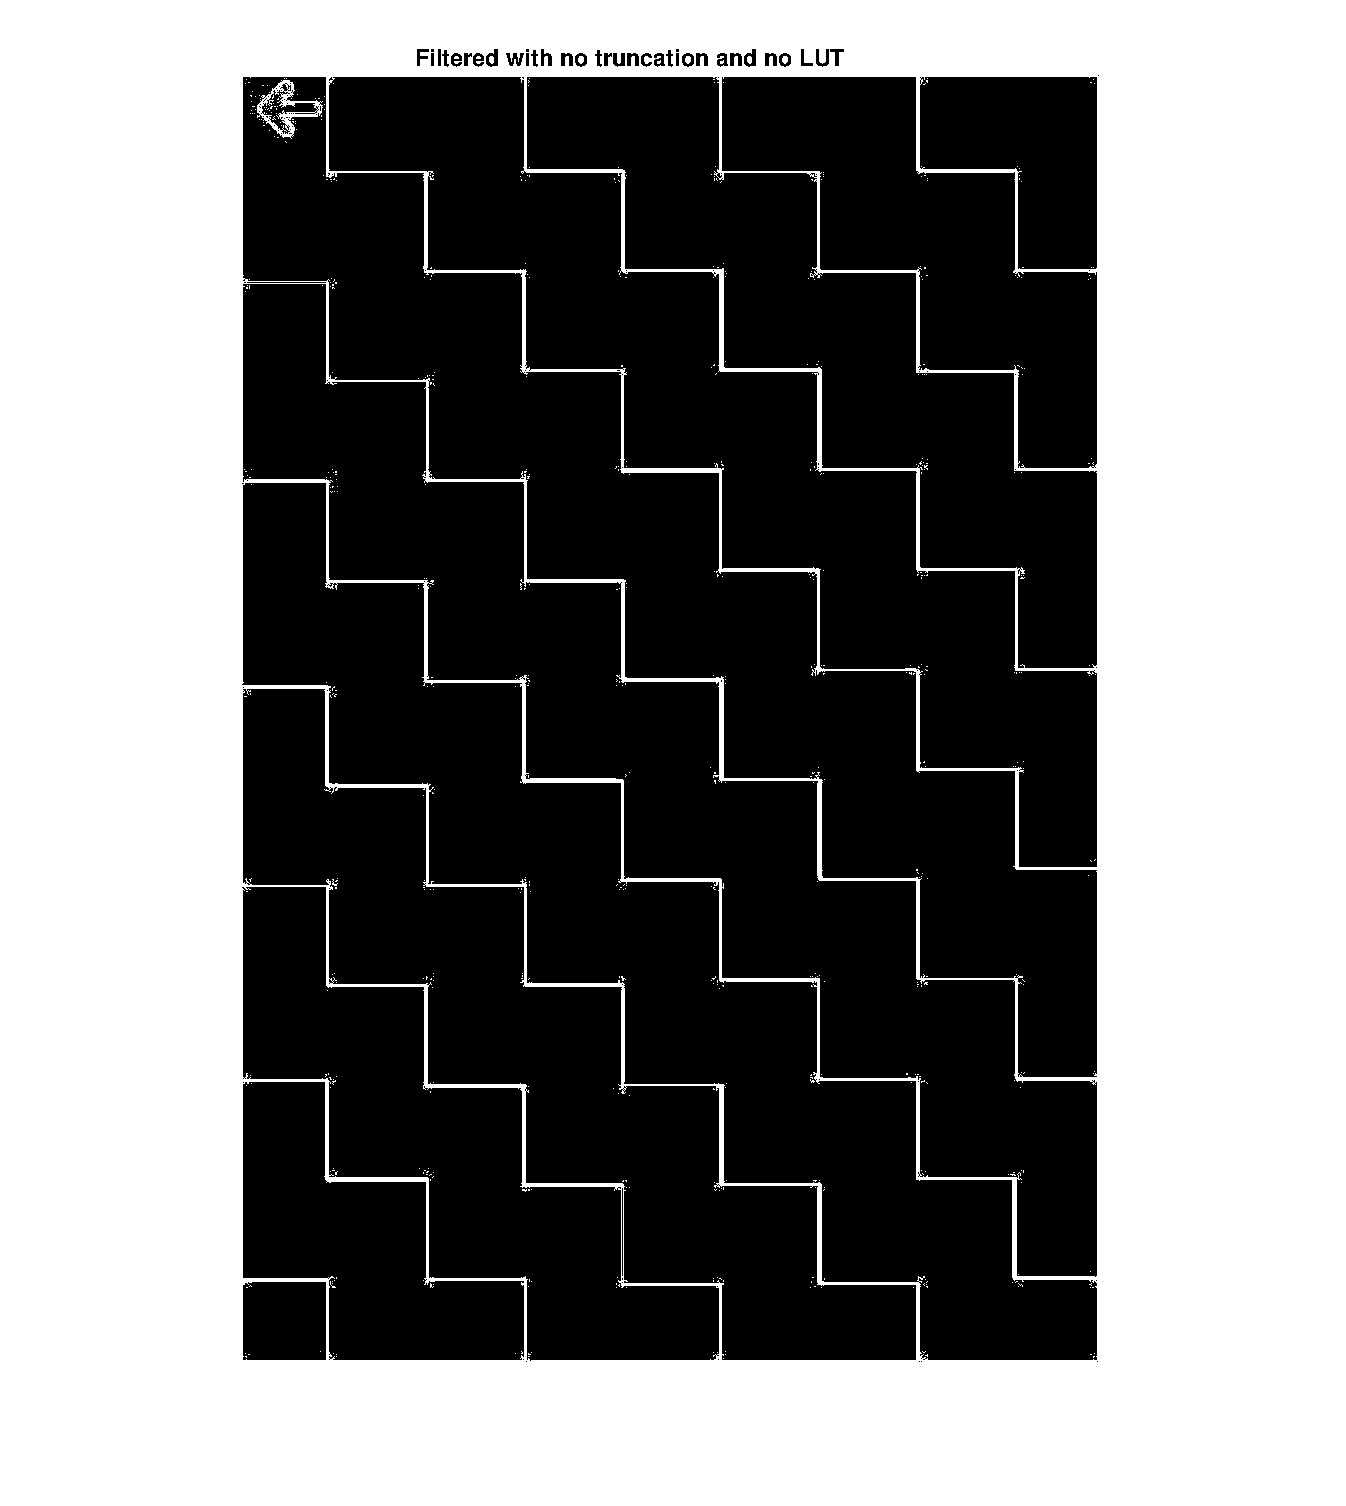
\includegraphics[width=140pt]{zigzag_HP.eps} \caption{Image after HP filter} \label{blahblah} \end{figure}}
\only<3>{\begin{figure}[h] 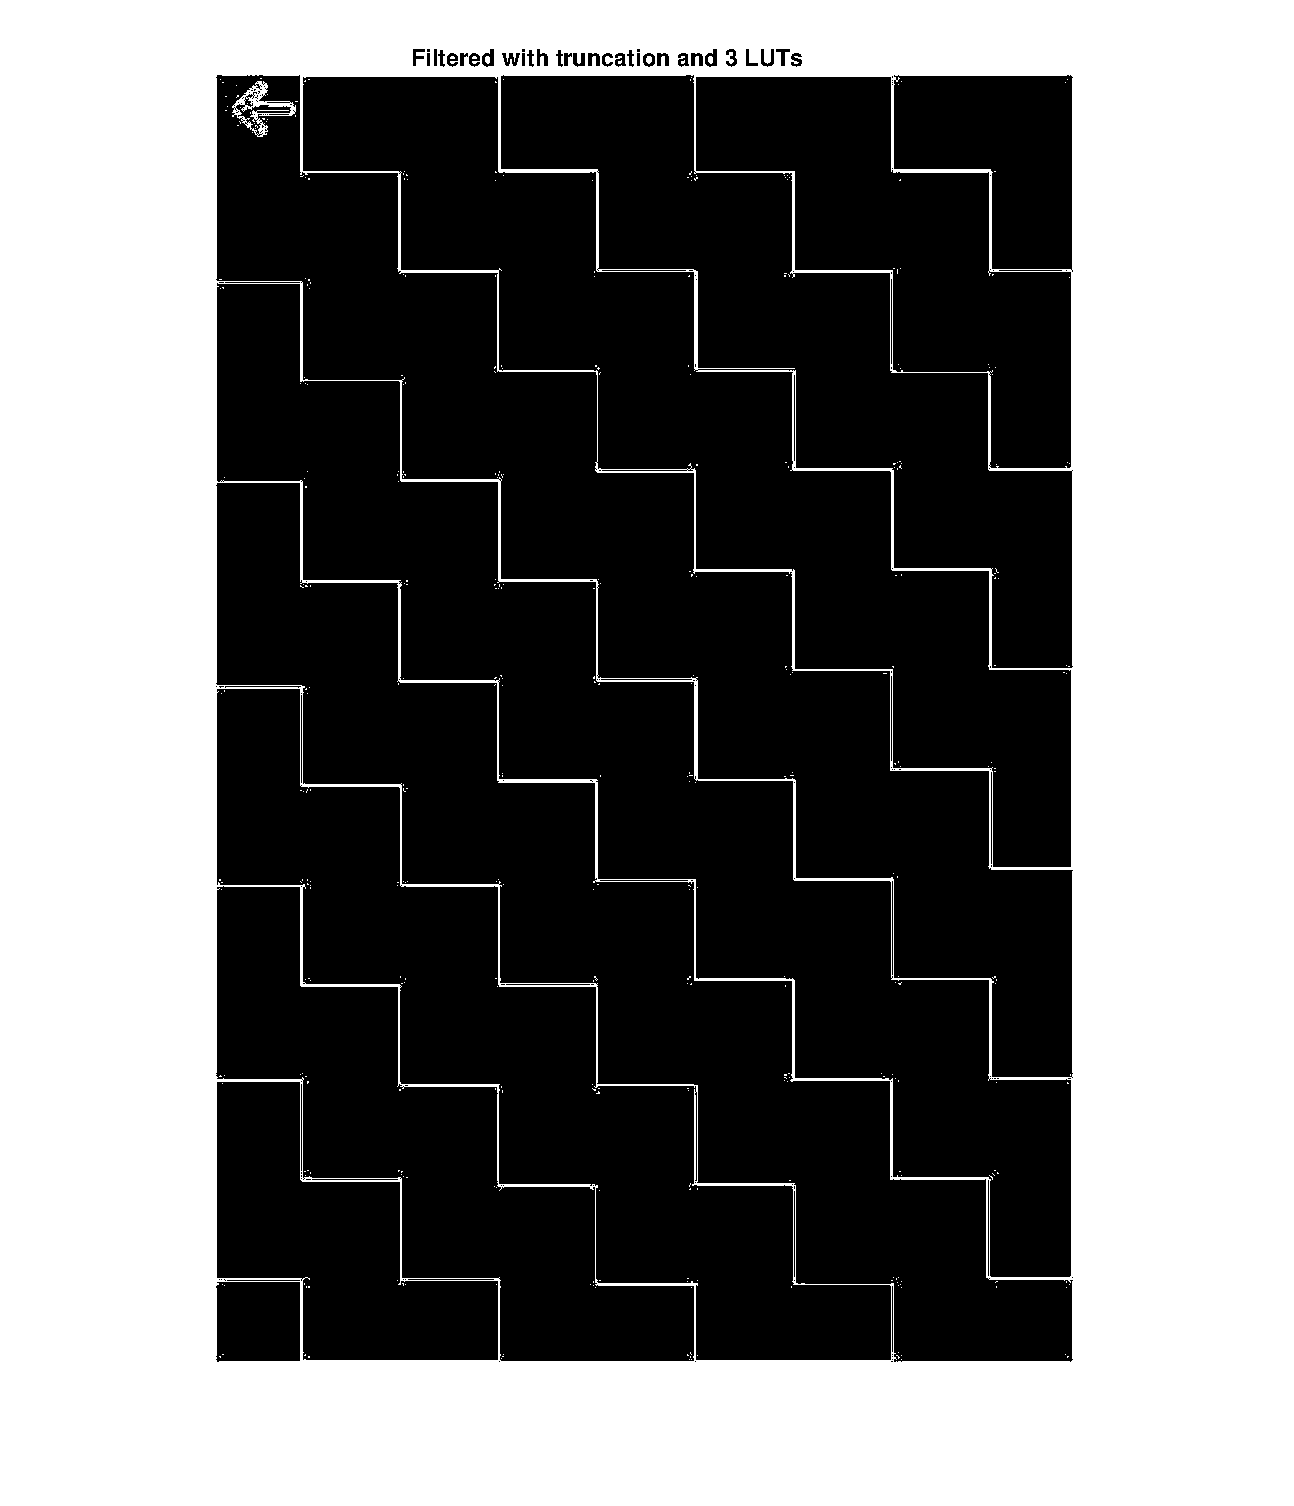
\includegraphics[width=140pt]{zigzag_HP_LUT_T.eps} \caption{Image after HP filter with 3 LUT's\\containing 16, 4096, and 16 entries} \label{blahblahblah} \end{figure}}
\end{frame}

\begin{frame}
\frametitle{Truncation and Blurring Filter (using Edge-detection filter)}
Observation
\begin{enumerate}
\item The truncation method can be used to reduce running time.
\item Truncation makes some errors such as staircase effects for blurring, but is decent for edge-detecting.
\end{enumerate}
\bigskip
\pause
\begin{center}
$\Downarrow$
\end{center}

\pause
\begin{beamerboxesrounded}[lower=eeks2,upper=eecks,
shadow=true]{Goal}
Take advantage of the truncation method avoiding staircase effects!
\end{beamerboxesrounded}
\end{frame}

\begin{frame}
\frametitle{Truncation and Blurring Filter (using Edge-detection filter)}

\begin{beamerboxesrounded}[lower=eeks2,upper=eecks,
shadow=true]{IDEA}
$I-L$ can be regarded as an edge-detection filter even though it is not a high-pass filter in general.
\end{beamerboxesrounded}

\begin{wrapfigure}{l}{0.3\textwidth}
\includegraphics[width=0.9\linewidth]{I-LPF.png} 
\caption*{Example of $I-L$.}
\end{wrapfigure}

\bigskip

\pause

Strategy

\begin{itemize}
\item[1.] Let $L$ be given low-pass filter.
\item[2.] Set $H:=I-L$. 
\item[3.] Find $I-H(T)$ for a certain truncation $T$.
\end{itemize}
\pause
\begin{center}
$\Downarrow$
\end{center}

\pause
$$L\approx I-H(T)$$
\end{frame}

\begin{frame}
\frametitle{Truncation and Blurring Filter (using Edge-detection filter)}
Let $$L=
\frac{1}{8}
\begin{bmatrix}
0 & 1 & 0\\
1 & 4 & 1\\
0 & 1 & 0
\end{bmatrix} \mbox{ and } T=\left[
\begin{array}{ccc}
8 & 6 & 8 \\
6 & 4 & 6 \\
8 & 6 & 8
\end{array}
\right].$$

\begin{figure}[h] \centering 
\begin{subfigure}[b]{0.3\textwidth} \includegraphics[width=\textwidth]{LPF.png} \caption{Low-pass filter, $L$} \end{subfigure}
\begin{subfigure}[b]{0.3\textwidth} \includegraphics[width=\textwidth]{truncation.png} \caption{Truncation, $L(T)$} \end{subfigure}
\begin{subfigure}[b]{0.3\textwidth} \includegraphics[width=\textwidth]{new.png} \caption{New Idea, $I-H(T)$} \end{subfigure}
\caption{Comparison of filtered images}%\label{fig:comp} 
\end{figure}

\end{frame}

\begin{frame}
 The table shows us how $L(T_i)$ and $I-H(T_i)$ are different from the low-pass filter $L=I-H$ for each $i$. $L(T_i)$ is Old and $I-H(T_i)$ is New in the table.

\begin{table}[ht]
\begin{center}
\begin{tabular}{c|c|c|c|c|c|c|}
\cline{2-7}  & \multicolumn{2}{|c|}{$T_{1}$} &
\multicolumn{2}{c|}{$T_{2}$} & \multicolumn{2}{c|}{$T_{3}$}
\\\cline{2-7} & Old & New & Old & New & Old & New \\\hline \multicolumn{1}{ |c| }{PSNR} &
38.12 & 39.58 & 30.80 & 32.84 & 22.59 & 25.59 \\\hline
\multicolumn{1}{ |c| }{$l_{2}$ - error} & 3.06 &  2.80 &  7.40 & 5.87 &
18.87 & 13.52 \\\hline \multicolumn{1}{ |c| }{$l_{\infty
}$ -
error} & 8.42 & 7.40 & 19.64 & 15.81 & 43.35 & 35.70 \\
\hline
\end{tabular}
\bigskip

\caption{Comparison of errors}
\end{center}
\end{table}
\end{frame}
\section{Further Directions}

\begin{frame}
\frametitle{Further Directions}
\begin{figure}[htb]
  \begin{center}
  \includegraphics[height=1.7in,angle=270]{group4.JPG}
  \caption{Eat more Punch pizza!}
  
  \end{center}
  \end{figure}
  
  
\end{frame}

\begin{frame}
\frametitle{ }
\begin{center}
{\huge Thank you!}
\end{center}
% Thank the IMA and our mentor Dr. Wu
% \begin{figure}
% \includegraphics[width=2in]{group.JPG}
% \includegraphics[width=2in]{group_rotated.JPG}
% \end{figure}
\end{frame}

\end{document}